\documentclass[a4paper]{report}
\setlength{\headheight}{12.0pt}
\usepackage[T2A]{fontenc}
\usepackage[utf8]{inputenc}
\usepackage[russian,english]{babel}
\usepackage[left=25mm, top=20mm, right=25mm, bottom=30mm, nohead, nofoot]{geometry}
\usepackage{amsmath,amsfonts,amssymb} % математический пакет
\usepackage{fancybox,fancyhdr}
\usepackage{xcolor}
\usepackage{hyperref}
\usepackage{tkz-euclide}
\usepackage{enumitem}
\usepackage{amsmath}
\usepackage{pgfplots}
\usepackage{float}
\usepackage{fvextra}
\usepackage[cache=false]{minted}
\usepackage[figurename=Изображение]{caption}
\captionsetup[table]{name=Таблица}
\usemintedstyle{vs}

\hypersetup{colorlinks=true, allcolors=[RGB]{010 090 200}} % цвет ссылок
\newcommand{\lr}[1]{\left({#1}\right)} % команда для скобок
\pagestyle{fancy}
\fancyhf{}
\renewcommand{\headrulewidth}{0pt}
\fancyfoot[R]{\thepage}
\fancypagestyle{plain}{
    \fancyhf{}
    \fancyfoot[R]{\thepage}
    \renewcommand{\headrulewidth}{0pt}
}
\setcounter{page}{1} % счетчик нумерации страниц
\headsep=10mm
\definecolor{green_india}{HTML}{138808} % INDIA GREEN
\definecolor{green_light}{HTML}{90EE90} % LIGHT GREEN
\definecolor{green_slimy}{HTML}{299617} % SLIMY GREEN
\makeatletter
\def\@seccntformat#1{\csname #1ignore\expandafter\endcsname\csname the#1\endcsname\quad}
\let\latex@numberline\numberline
\def\numberline#1{\if\relax#1\relax\else\latex@numberline{#1}\fi}
\makeatother
\renewcommand{\thesection}{\arabic{section}.}
\renewcommand{\thesubsection}{\arabic{section}.\arabic{subsection}}

\begin{document}
\section{Диаграмма вариантов использования}
\subsection{Дикоед}
\begin{figure}[H]
    \centering
    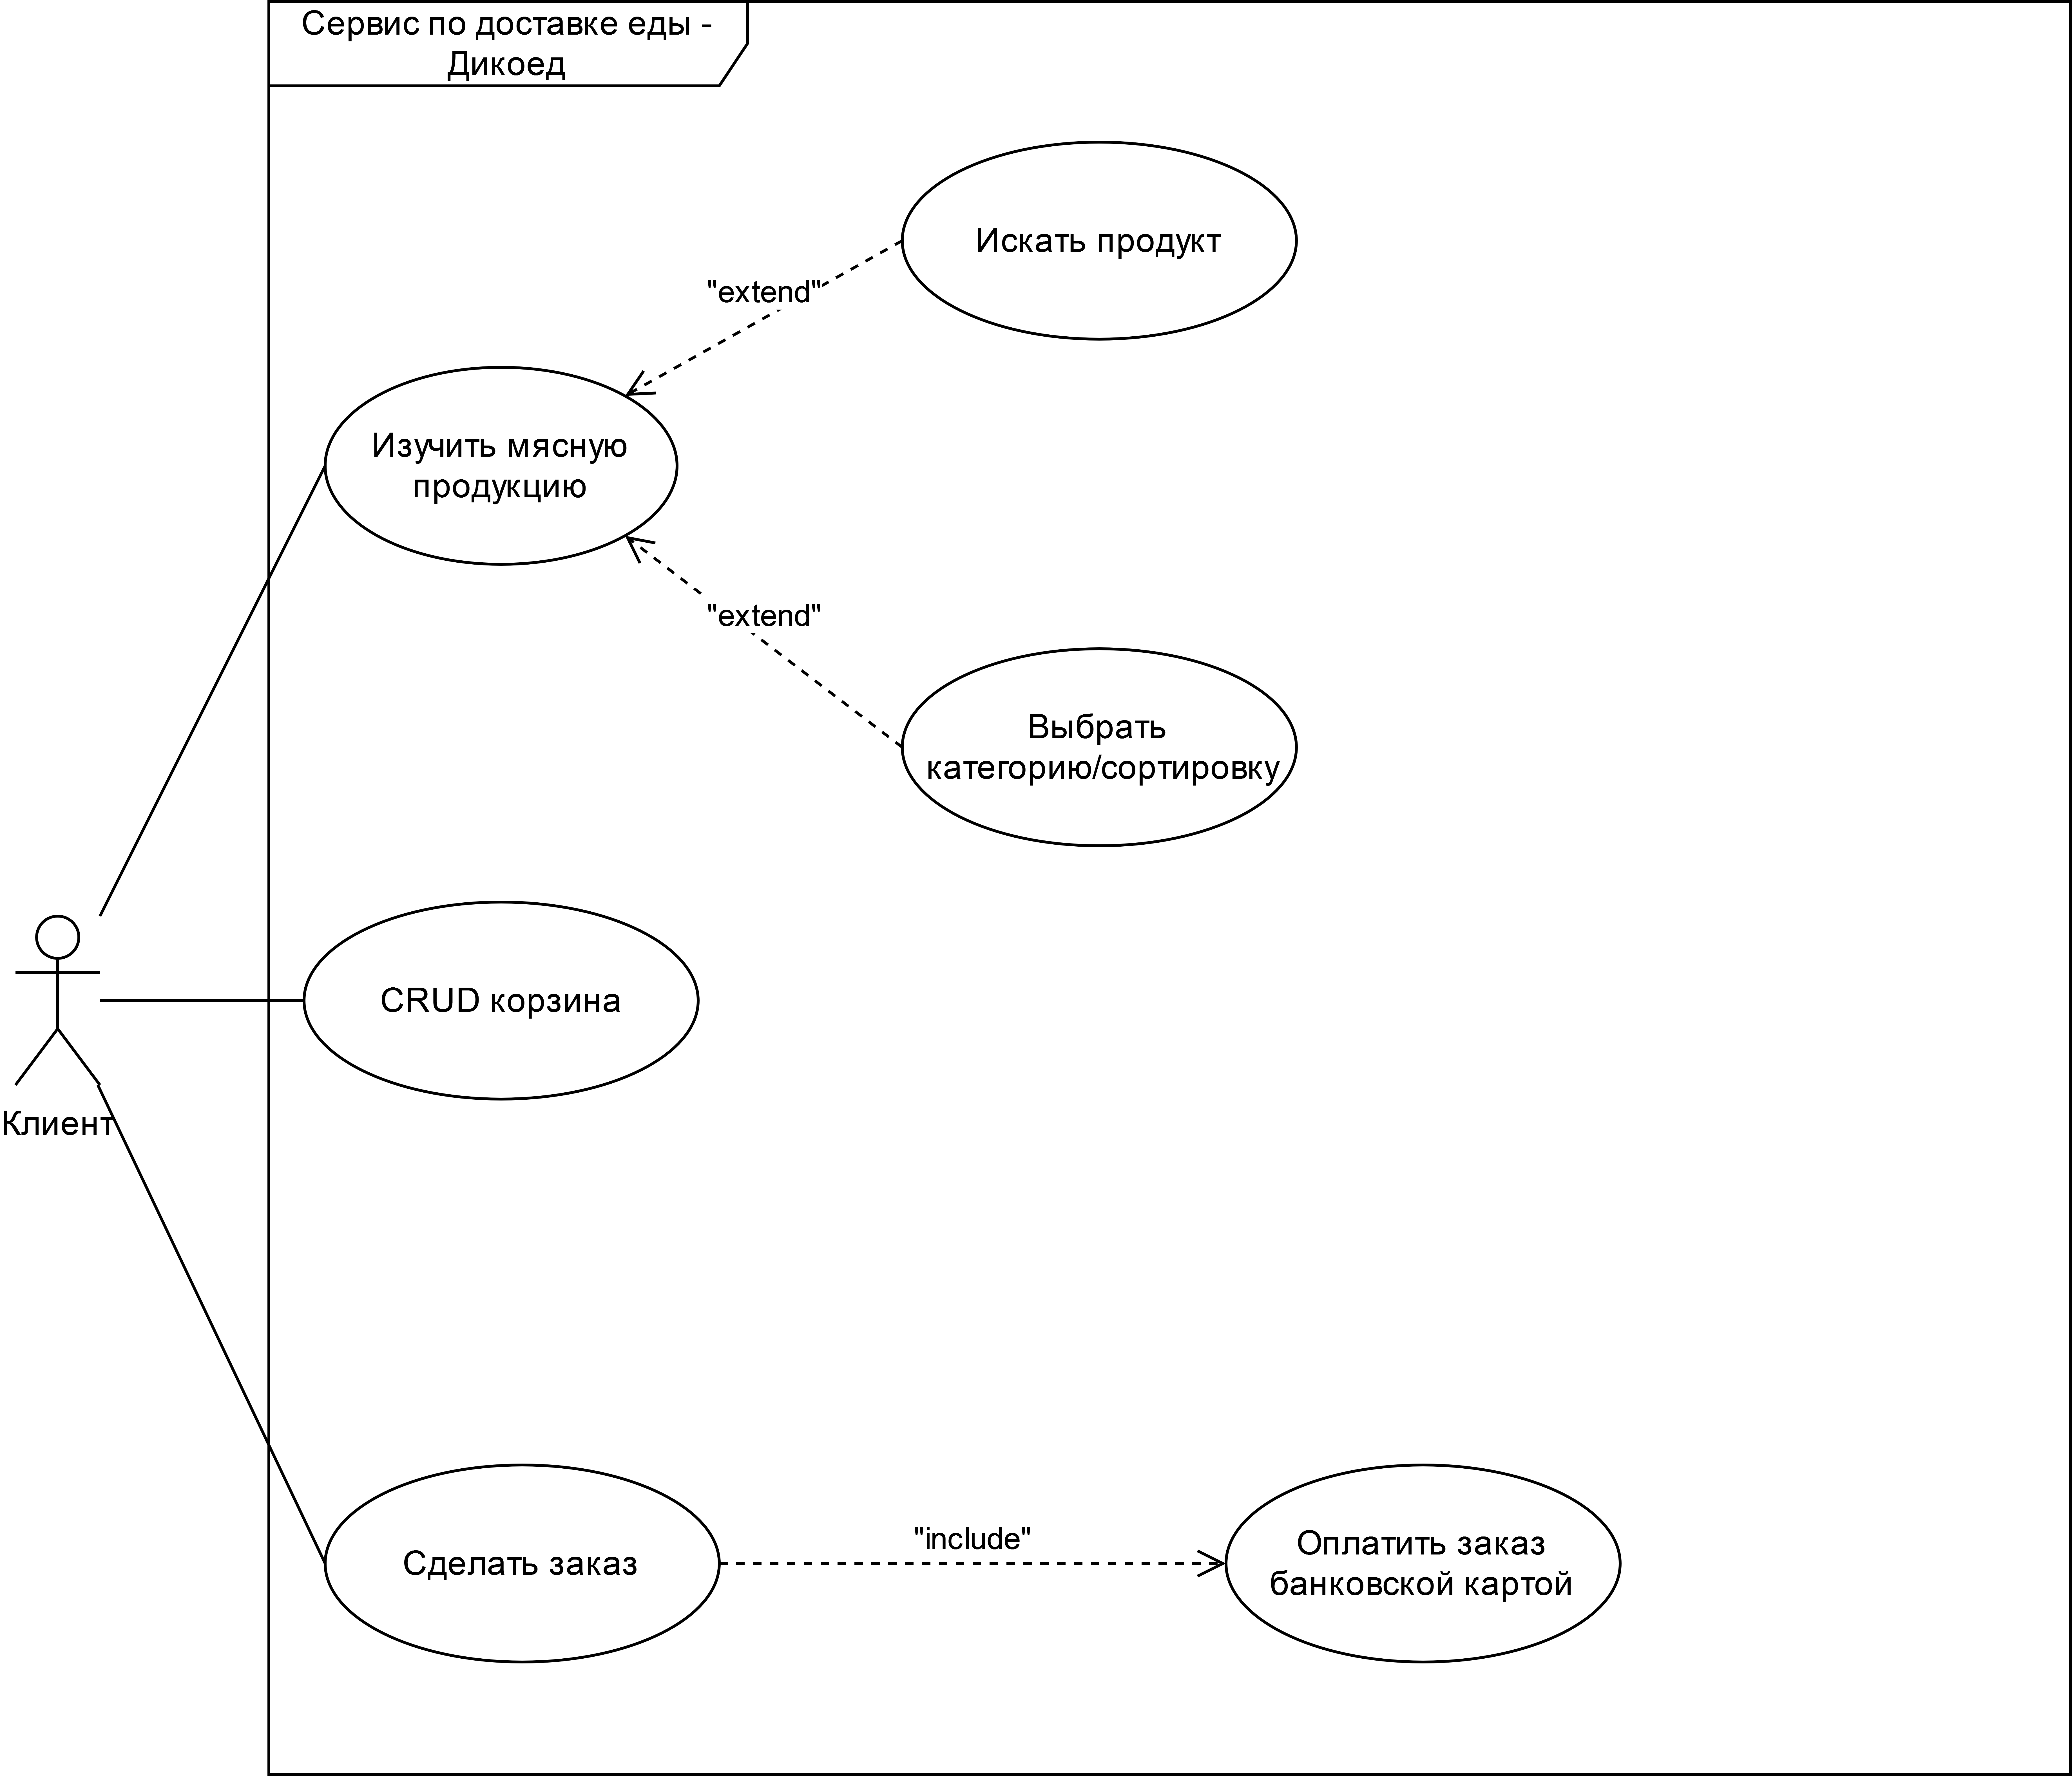
\includegraphics[width=\textwidth]{Диаграмма вариантов использования Дикоед.png}
\end{figure}
\subsection{Самокат}
\begin{figure}[H]
    \centering
    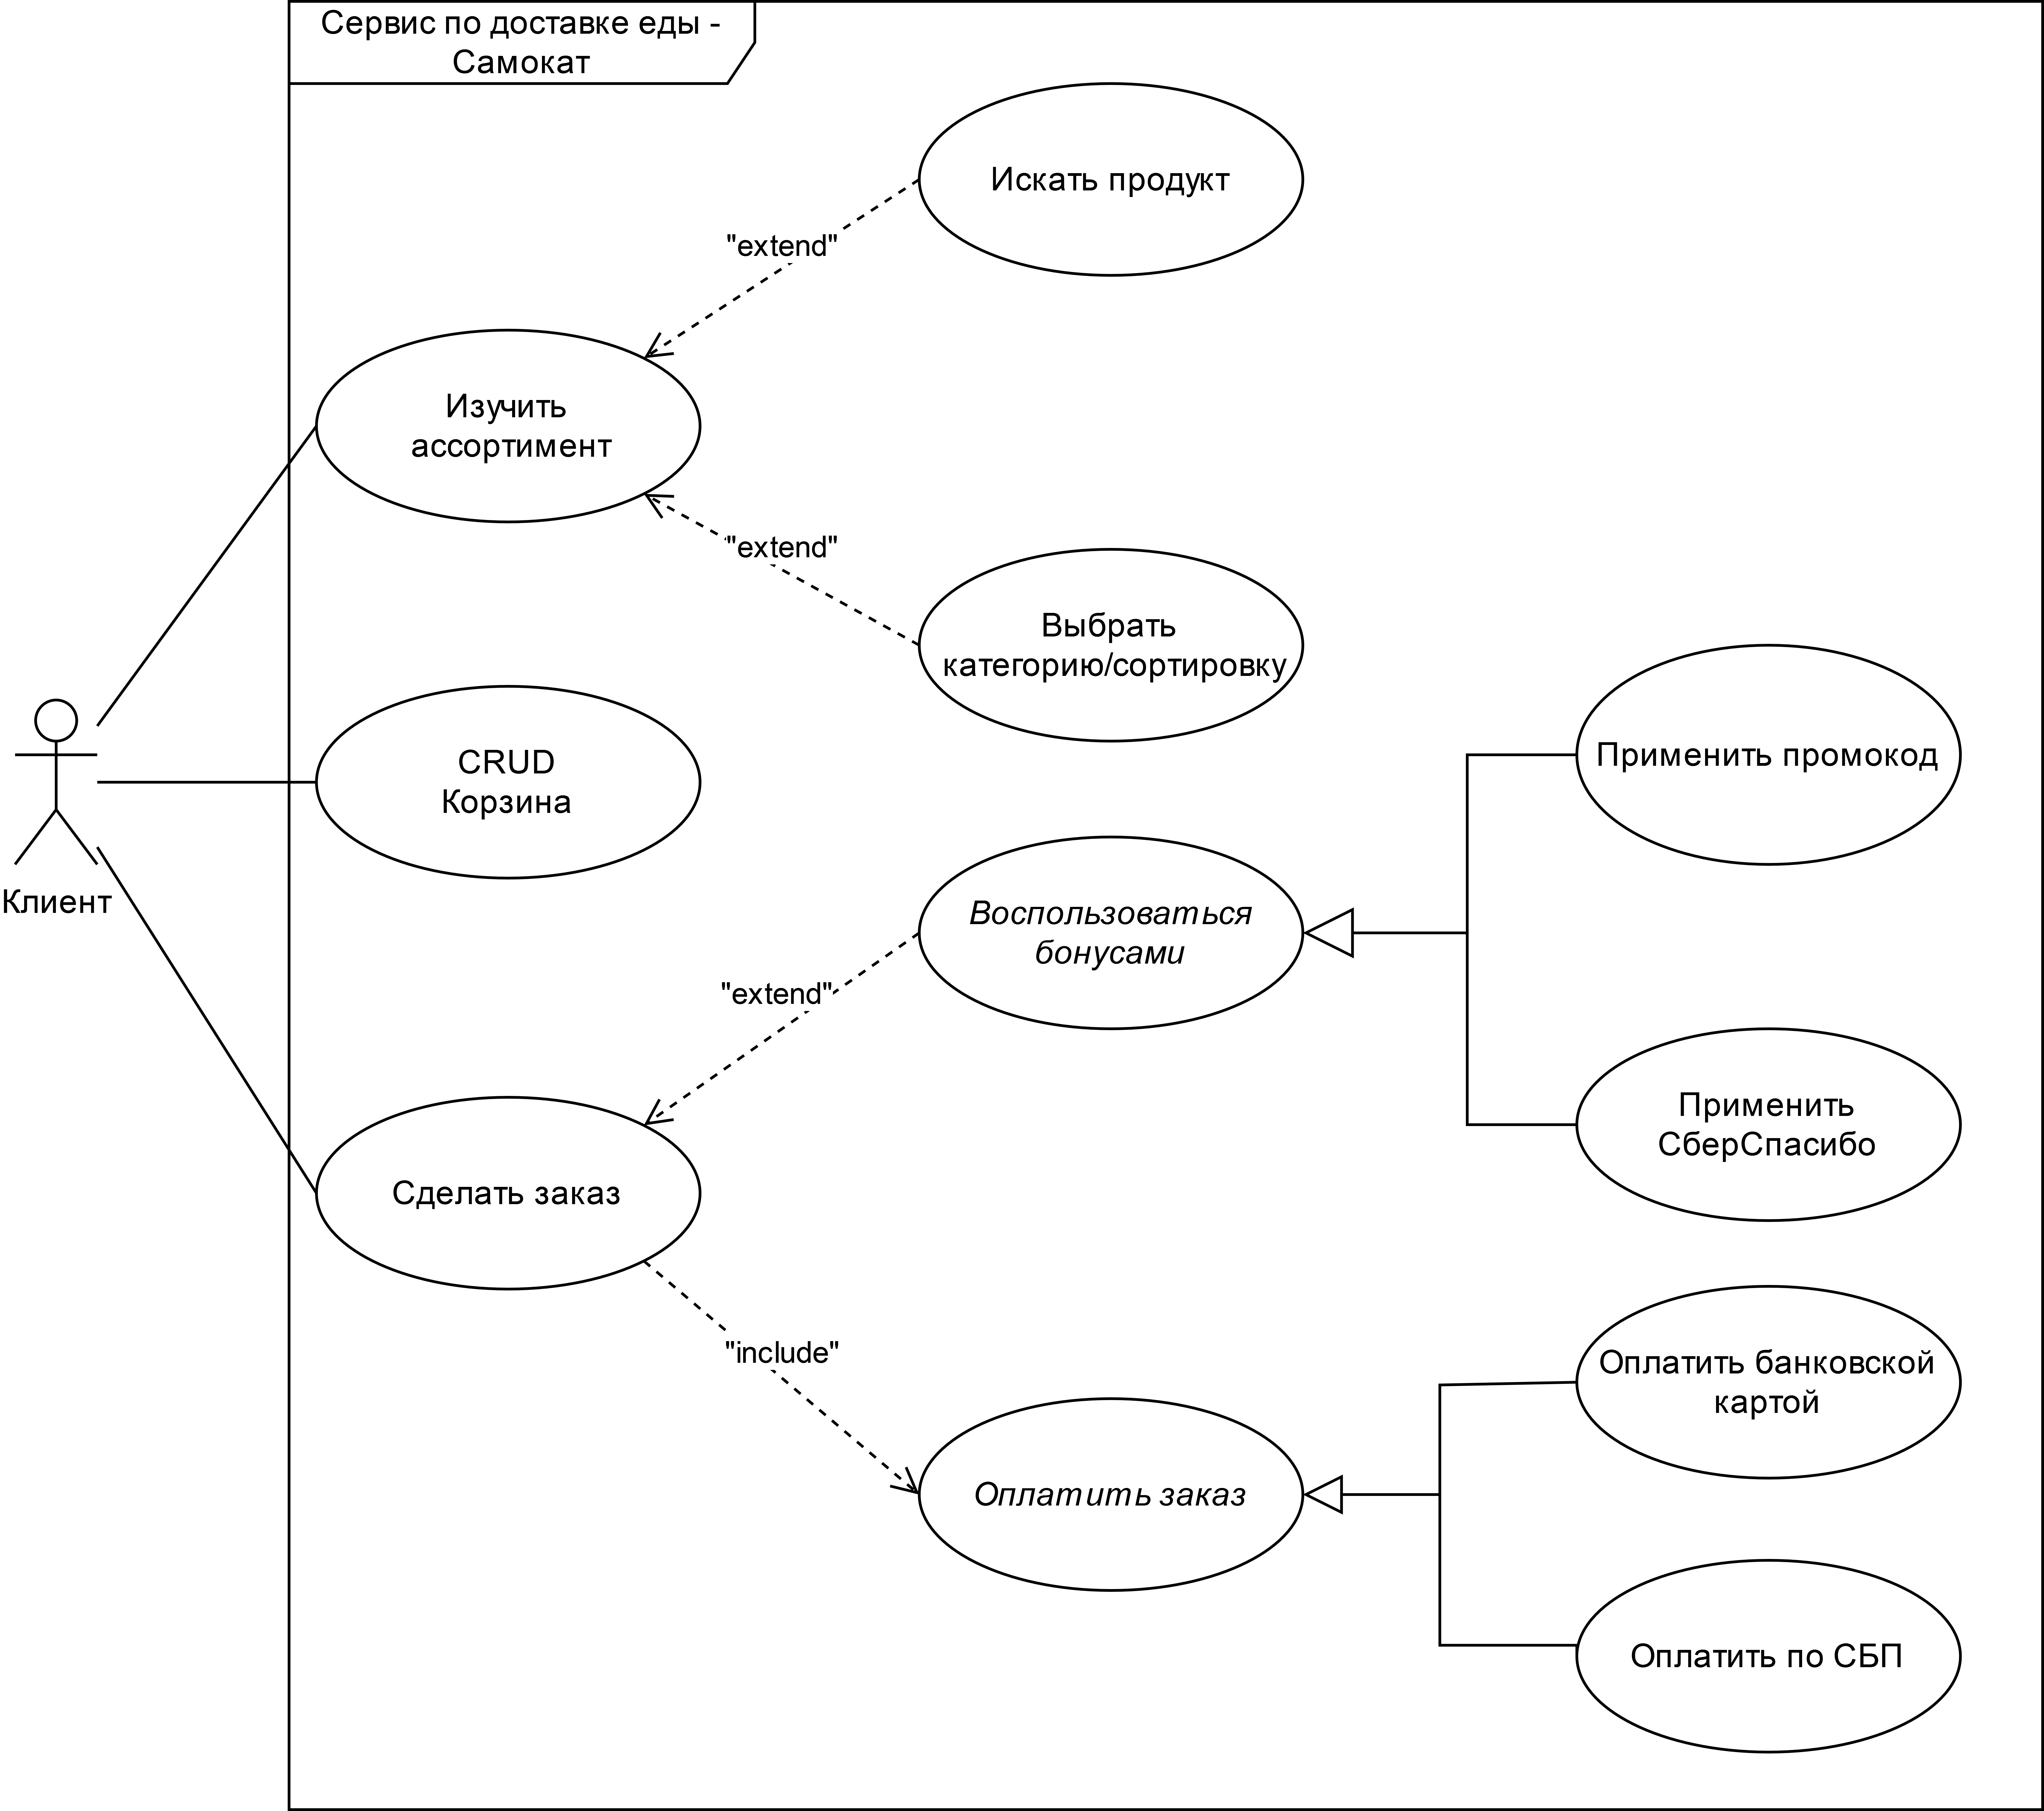
\includegraphics[width=\textwidth]{Диаграмма вариантов использования Самокат.png}
\end{figure}
\newpage
\subsection{Сервис по продаже фермерской продукции}
\begin{figure}[H]
    \centering
    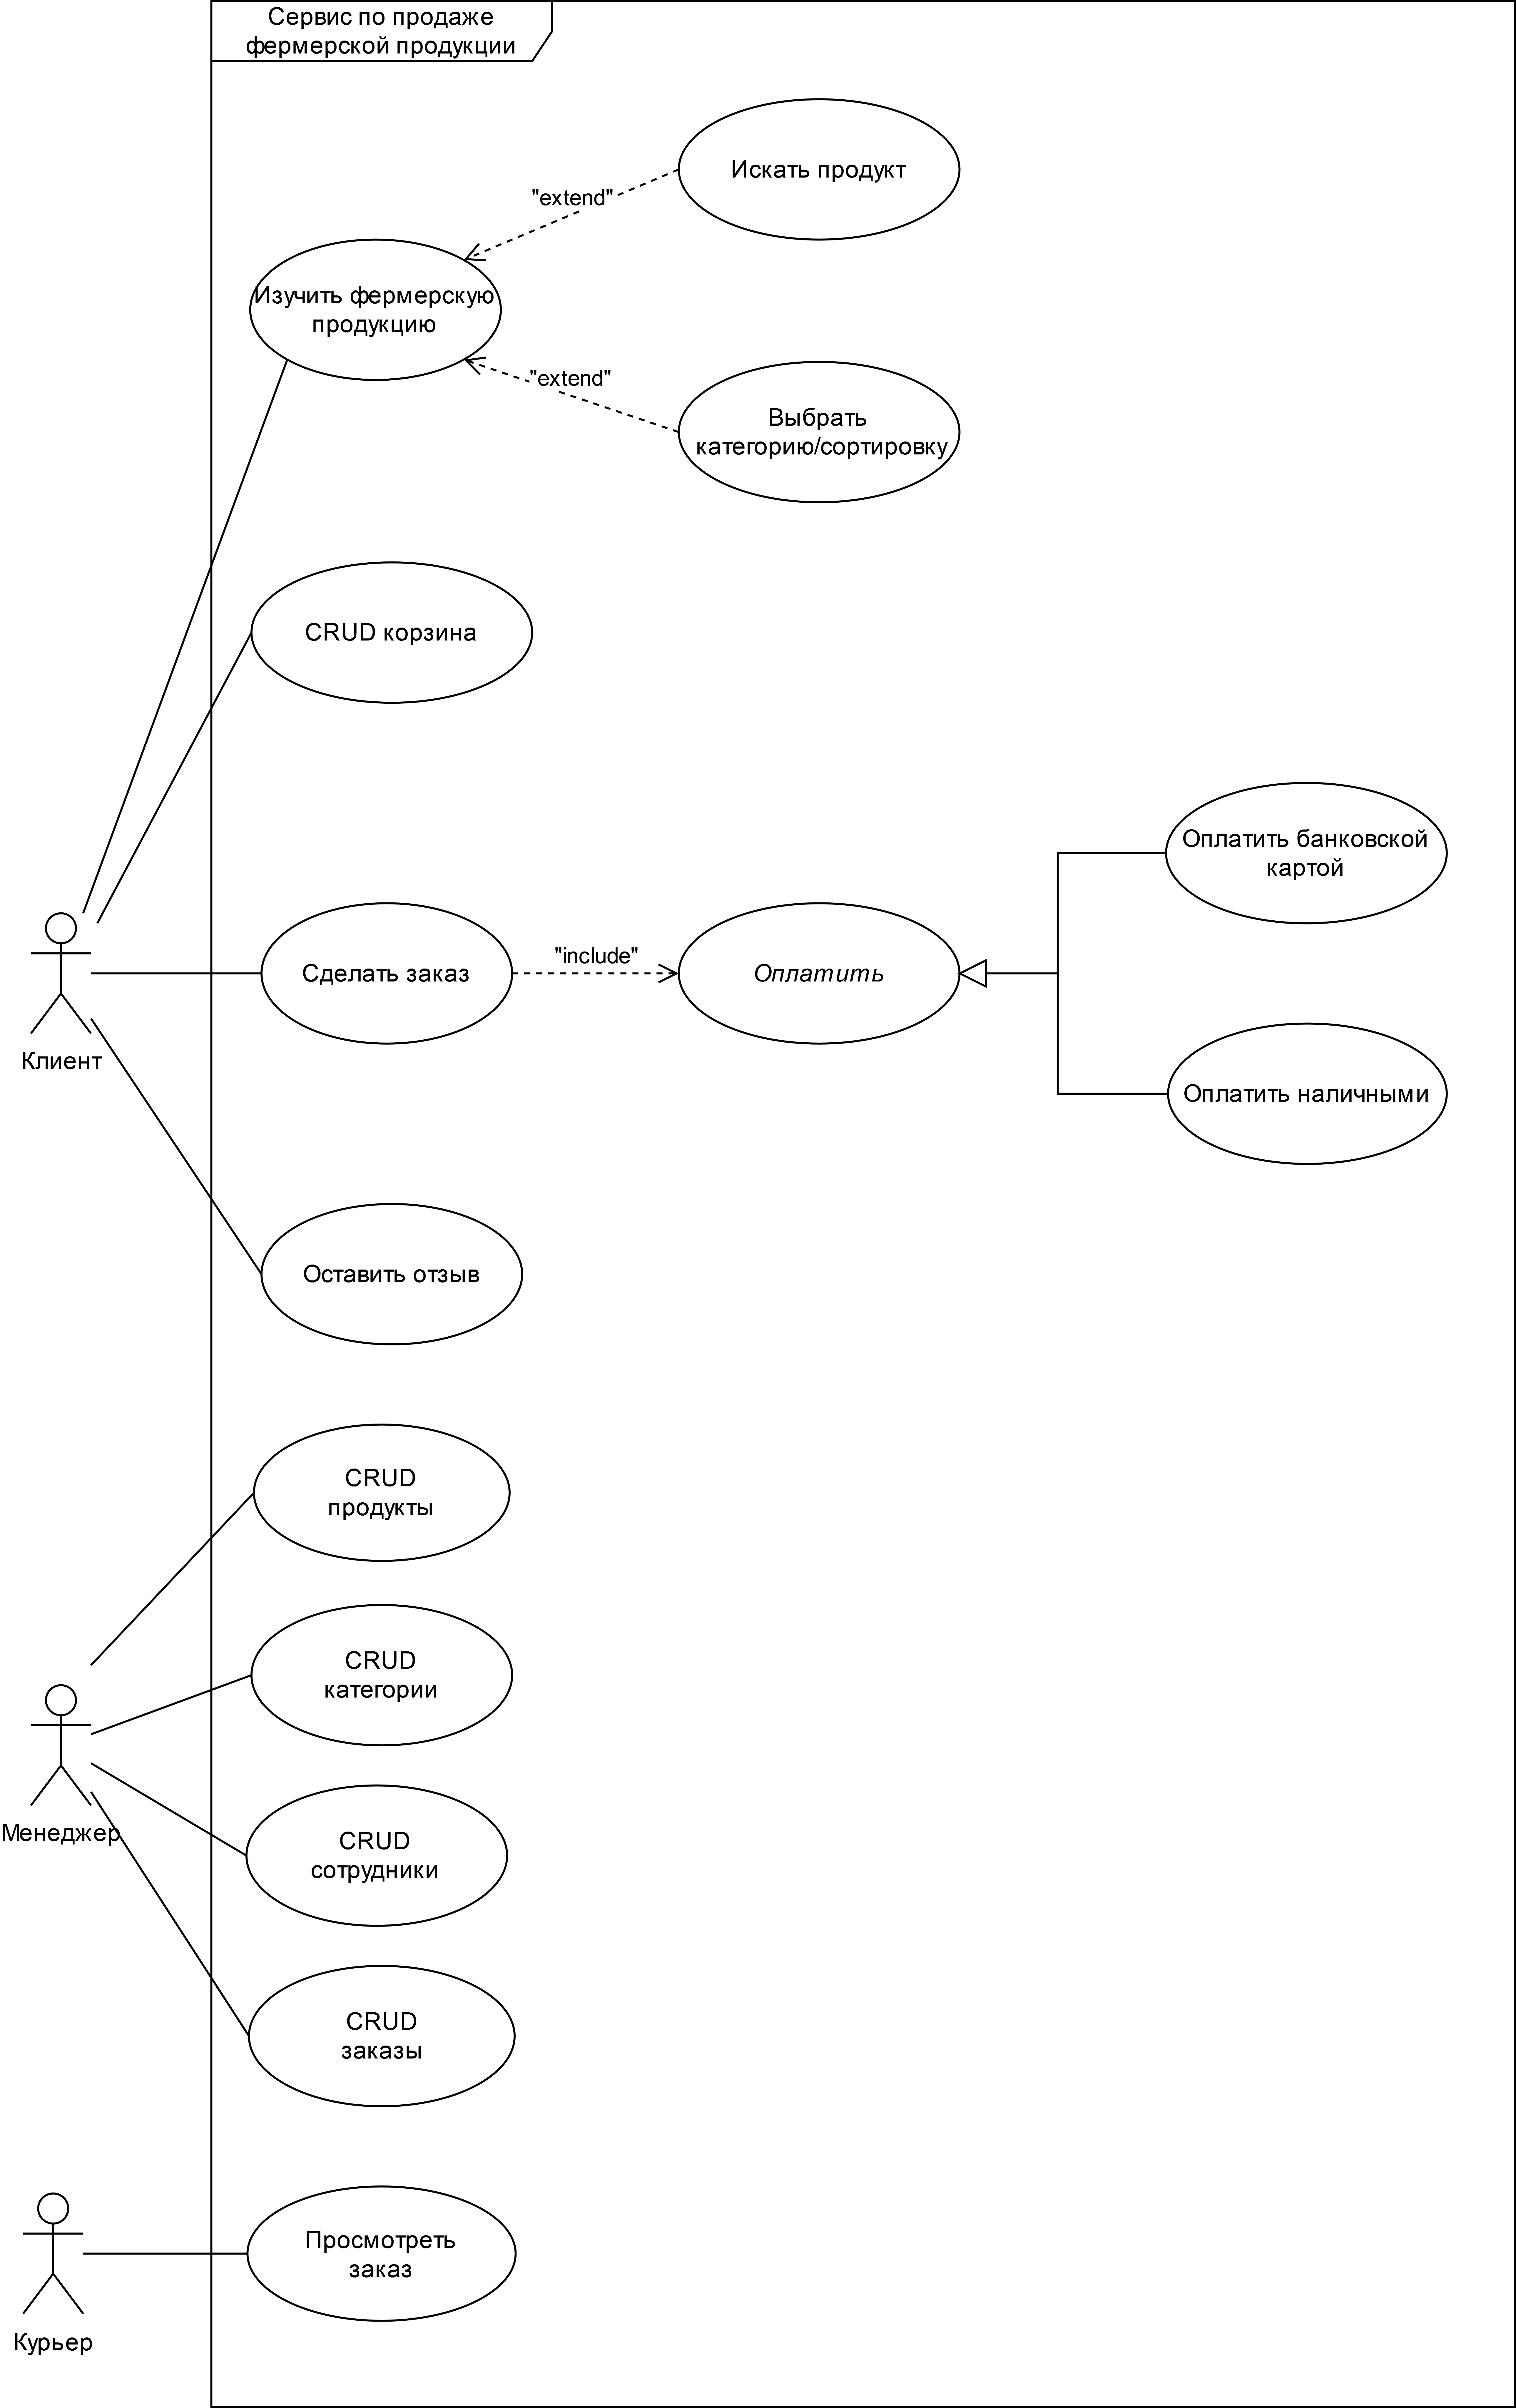
\includegraphics[height=0.9\textheight]{Диаграмма вариантов использования Сервис по продаже фермерской продукции.png}
\end{figure}
\subsection*{Основные действия пользователей}
\begin{enumerate}
    \item Изучить фермерскую продукцию\begin{enumerate}
        \item Искать продукт;
        \item Выбирать категорию/сортировку;
        \item CRUD корзину.
    \end{enumerate}
    \item Сделать заказ\begin{enumerate}
        \item Указать адрес доставки;
        \item Выбрать дату доставки;
        \item Выбрать способ оплаты\begin{enumerate}
            \item Оплатить банковской картой;
            \item Оплатить наличными.
        \end{enumerate}
        \item Выбрать способ получения\begin{enumerate}
            \item Самовывоз;
            \item Доставка
        \end{enumerate}
    \end{enumerate}
    \item Оставить отзыв
\end{enumerate}
\subsection*{Действия администраторов/сотрудников}
CRUD действия для управления системой.
\subsection*{Общие элементы}
Возможность <<Просмотреть заказ>> как дополнительная функция.
\newpage
\subsection*{Сценарий <<Сделать заказ>>}    
\textbf{Описание:} пользователь желает приобрести товары из корзины, получить свой заказ и осуществить платеж.\\\\
\textbf{Предусловие:} Покупатель находится на странице с корзиной. В корзину добавлен один и более товаров.\\\\
Основной сценарий:
\begin{enumerate}
    \item Покупатель выбирает команду «Перейти к оформлению заказа»;
    \item Система открывает страницу «Оформление заказа»;\\Примечание: по умолчанию способ доставки – «доставка на дом».
    \item Покупатель вводит адрес доставки и выбирает команду «Далее»;
    \item Система открывает страницу «Выбор даты доставки»;
    \item Покупатель выбирает дату доставки и нажимает команду далее;
    \item Система открывает страницу «Выбор способа оплаты»;
    \item Покупатель выбирает способ оплаты и нажимает команду далее;
    \item Система открывает страницу заказа со всей информацией о заказа;
    \item Покупатель выбирает команду «подтвердить»;
    \item Система открывает страницу заказа со статусом «заказ сформирован».
\end{enumerate}
$$$$\\\\
Альтернативный сценарий 1:
\begin{enumerate}
    \item Заменяет шаг 3 Основного сценария. Начинается, когда на шаге 3 Покупатель выбирает способ получения «Самовывоз»
    \begin{enumerate}
        \item Система открывает страницу «Самовывоз» на которой присутствует адрес и карта на которой отмечено местоположение пункта самовывоза;
        \item Покупатель нажимает «Далее».
    \end{enumerate}
\end{enumerate}
\end{document}